\chapter{Vizualizace dat}
\label{ch:vizualizace}

Očištěná data vybrané společnosti obsahující záznamy shrinků, které byly způsobeny škodami, jsem vizualizovala v nástroji Power BI, který se používá pro business intelligence analýzu. Vytvořila jsem report, který umožňuje pomocí interaktivních grafů analyzovat data. První část této kapitoly se věnuje technickému popisu reportu, zatímco druhá část shrnuje výsledky analýzy plynoucí z reportu.

\section{Popis řešení}
\label{sec:vizualizace:popis}

Report obsahuje pět stránek. První stránka nabízí základní přehled, dashboard, týkající se všech shrinků. Druhý list je věnován prodejnám a údajům o lokalitách.
Další stránky se již věnují pouze shrinkům zaviněných škodami a kategoriím Velmi čerstvé a Čerstvé z produktové hierarchie úrovně 1. Třetí list zobrazuje hodnoty ukazatelů hodnoty shirnku a odvozených podílů. Na čtvrtém a pátém listu jsou další přehledy z pohledu konkrétních produktů, kategorií a typů promoakce. Poslední stránka týkající se reportingu je z pohledu vybraného konkrétního produktu.

Do Power BI souboru jsem pomocí integrovaného nástroje PowerQuery nahrála upravená data z databáze vybrané společnosti. Hlavní faktickou tabulkou je tabulka \emph{damages}, která obsahuje všechny zaznamenané shrinky z kategorie shrinků, které byly způsobeny škodami. Druhá faktická tabulka má název \emph{revenue} a obsahuje tržby v pozorovaném měsíci pro všechny prodejny, tržby jsou dále rozdělené podle kategorie z úrovně 1 a do čtvrtin měsíce. Doménové tabulky jsou číselník produktů, číselník shrinků a číselník prodejen, dále také číselníkové tabulky, které spojují faktické tabulky -- čtvrtina měsíce a seznam kategorií úrovně 1. 

Datový model tabulek, které jsou vstupem do reportu je znázorněný na obrázku \ref{obr:datmod}. Mezi jednotlivými tabulkami jsou znázorněny vazby -- jejich mohutnost a směr. Tabulka \emph{metrics}, která není navázaná na žádnou jinou tabulku obsahuje výpočetní metriky, které vychází z dat v modelu, metriky se dále používají ve vizualizacích.

\begin{figure}[hbtp!]
    \centering
    \captionsetup{justification=centering}
    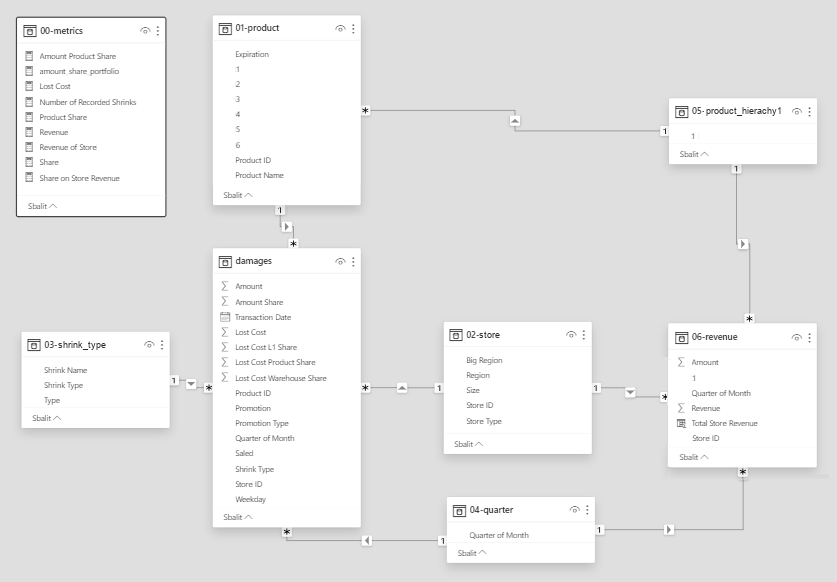
\includegraphics[width=\textwidth]{obrazky/PBI/datmodel.png}
    \caption{Datový model tabulek v Power BI reportu.}
    \label{obr:datmod}
\end{figure}

Reporting je zpracován v angličtině, takže i dříve popsané názvy kategorií nebo shrinků jsou přeložené. Překlad je uvedený v příloze práce. Uvedené tržby v reportingu odpovídají nekonkrétní peněžní jednotce -- z důvodu ochrany dat vybrané společnosti byla skutečná čísla vynásobena jistým koeficientem. Poměry zobrazené v reportu ale vstupním datům společnosti odpovídají.

\subsection{Metriky}

Power BI nabízí uživatelům reportu širokou interakci s vizuály. Díky metrikám se zobrazené hodnoty přepočítávají podle aktuálních filtrů nebo podle vybraných dat. 

\begin{itemize}
    \itemsep-0.3em
    \item     \textbf{Lost Cost} -- Základní metrika s hodnotou shrinku ze vstupních dat.
    \item     \textbf{Product Share} -- Základní metrika, obsahuje podíl shrinku na tržbách produktu (přímo ze vstupních dat). Pokud je ve vizuálu agregovaná např. na kategorii nebo prodejnu, vypočítá se její průměr.
    \item     \textbf{Share} -- Základní metrika, obsahuje podíl shrinku na tržbách produktu. Pokud je ve vizuálu agregovaná na prodejnu jedná se celkový evidovaný shrink prodejny dělený tržbou dané prodejny. Pokud je agregovaný podle typu shrinku jedná se o podíl součtu hodnot všech záznamů daného typu a tržeb všech prodejen. Bude-li agregace probíhat zároveň na typu shrinku a na kategorii z úrovně 1, pak je podíl spočítaný vzhledem k této kategorii typu shrinku zároveň. 
    \item     \textbf{Share on Store Revenue} -- Základní metrika, obsahuje podíl shrinku na celkových tržbách produktu. Tj. pokud je agregace např. podle prodejny a podle kategorie jedná se o podíl všech shrinků produktu z dané kategorie vydělený celkovými tržbami vybrané prodejny. (Zatímco v předchozí metrice by se jednalo o tržby pouze za vybranou kategorii.)
    \item     \textbf{Revenue of Stores} -- Celková tržba prodejny za celé sledované období
    \item     \textbf{Revenue} -- Základní metrika s hodnotou tržeb prodejny rozdělená podle části měsíce podle kategorií z úrovně 1 a  ze vstupních dat.
    \item     \textbf{Number of Recorded Shrinks} -- Počet záznamů shrinků.
\end{itemize}

\subsection{Reporting}

\subsubsection*{Přehled}

První list obsahuje přehled týkající se všech typů shrinků v rámci kategorie shrinky způsobené škodami, přehled je v tabulce \ref*{tab:sh:dam} v kapitole \ref*{ch:shrinky}. Na obr. \ref*{obr:PBI:overview} je snímek tohoto listu, pro lepší orientaci při popisu jsem na snímek přidala označující čísla. Na této stránce jsou vyfiltrované všechny kategorie, shrinky i prodejny. V levé části jsou uvedeny souhrnné informace pro vyfiltrované záznamy (tj. implicitně nic vyfiltrováno není, jedná se o celkové hodnoty) (č. 1). 
Na grafu označeném č. 2, je znázorněno jak velký podíl shrinku na tržbách mají jednotlivé kategorie. Zároveň je barevně označeno, jakou měrou je hodnota zastoupená na malých či velkých prodejnách. Defaultní nastavení vizuálu je zobrazení kategorií úrovně 1, díky funkcionalitě nástroje Power BI je možné postoupit v hierarchii kategorií níže viz \ref*{obr:PBI:drill}. První graf zobrazuje defaultní pohled, na druhém je vidět výsledek pokud uživatel klikne na ikonu $\downdownarrows$ \emph{přechod k podrobnostem všech polí}. V takovém případě se postoupí na další úroveň hierarchie napříč všemi kategoriemi. Třetí graf ukazuje stav, kterého uživatel docílí, pokud zaklikne ikonu $\downarrow$ \emph{přechod k podrobnostem jednoho pole}\footnote{Anglicky se přechod k podrobnostem jednoho pole v nástroji Power BI označuje jako \emph{drill down}.}. V takovém případě, poté co uživatel klikne na jednu z kategorií v grafu (její název nebo příslušný datový pruh), se zobrazí nižší úroveň hierarchie, ale pouze takové kategorie, které jsou podkategorií vybrané kategorie. 
Další graf (č. 3) ukazuje jaký je podíl shrinku na tržbách pro malé a velké prodejny. V tomto vizuálu po zvolení přechodu k podrobnostem se rozbalí hodnoty podílu pro jednotlivé typy shrinků. Opět jako v předchozím případě lze postupovat buď pouze pro jeden typ prodejen nebo oba.
Pokud uživatel nezvolí \emph{přechod k podrobnostem jednoho pole} ve vizuálu, ale klikne na datový element ve vizuálu, všechny vizuály na listu se křížově vyfiltrují nebo křížově zvýrazní. Rozdíl mezi těmito dvěma akcemi je v sekci \ref*{sec:PBI}. 
\begin{figure}[hbtp!]
    \centering
    \captionsetup{justification=centering}
    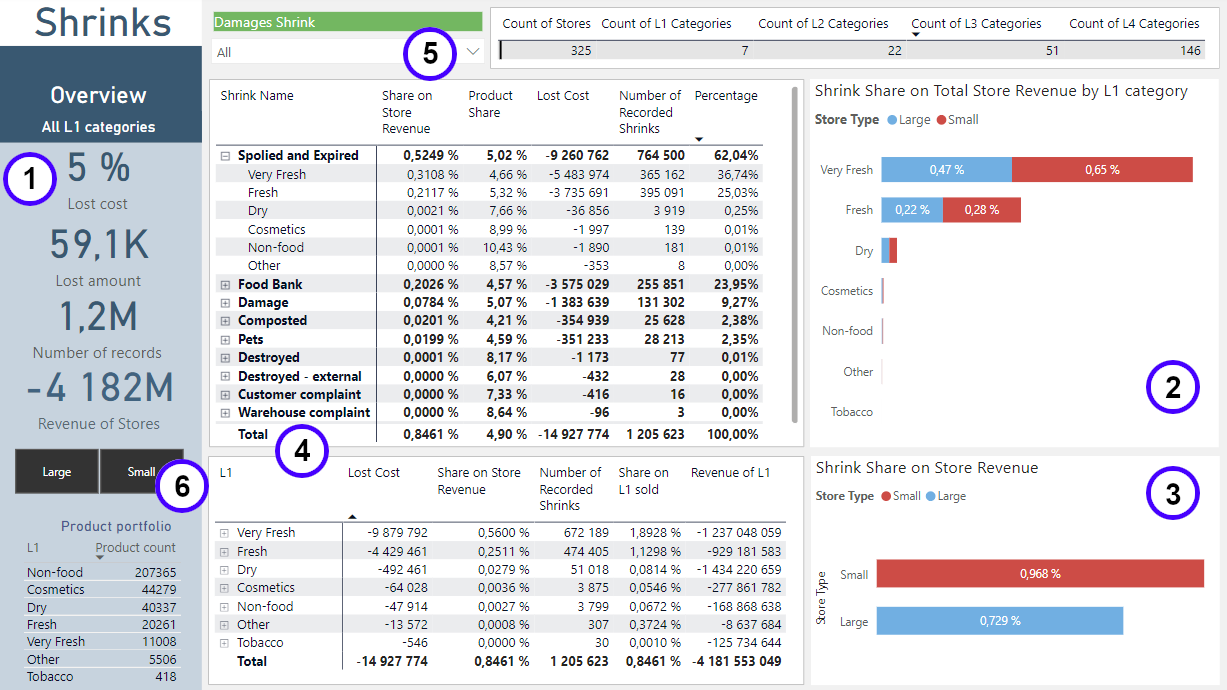
\includegraphics[width=\textwidth]{obrazky/PBI/overview.png}
    \caption{Power BI reporting pro zobrazení údajů o shrincích.}
    \label{obr:PBI:overview}
\end{figure}

Přehledový list dále obsahuje dvě tabulky. První tabulka sleduje vybrané ukazatele pro typy shrinků, které lze dále prozkoumat z pohledu kategorií první úrovně. Druhá tabulka zobrazuje ukazatele z pohledu kategorií, a to od nejvyšší úrovně po nejnižší, případně až na detail samotných produktů a jejich ID. Vzhledem k tomu, že tabulka může při detailním procházení zabírat více místa je možné přejít na její detail, který se zobrazí přes celý aktuální list. Ukázka této tabulky je na obr. \ref*{obr:PBI:tab1}.
U čísel 5 a 6 jsou umístěny filtry -- pro typ prodejny a pro typ shrinku. Vyfiltrováním příslušného typu se hodnoty v reportingu automaticky upraví. Všechny nevybrané kategorie nejsou zahrnuté do vizuálů, ani výpočtů hodnot. Např. pokud uživatel vybere pouze velké prodejny, celkové tržby se týkají již pouze všech velkých prodejen, nejde o celkové tržby všech prodejen z datasetu.

\begin{figure}[hbtp!]
    \centering
    \captionsetup{justification=centering}
    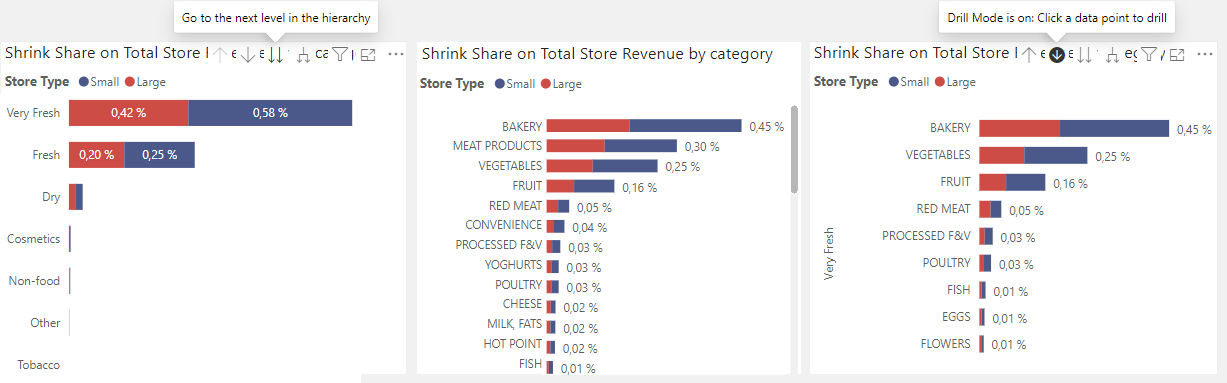
\includegraphics[width=\textwidth]{obrazky/PBI/Catdrilldown.png}
    \caption{Ukázka interakce grafu záznamů shrinku pro přístupy k různým úrovním produktové hierarchie.}
    \label{obr:PBI:drill}
\end{figure}

\begin{figure}[hbtp!]
    \centering
    \captionsetup{justification=centering}
    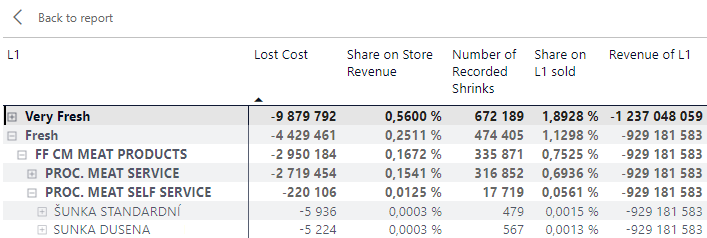
\includegraphics[width=\textwidth]{obrazky/PBI/tabulkaukzka.png}
    \caption{Detail tabulky vybrané ukazatele pro jednotlivé kategorie v produktové hierarchii.}
    \label{obr:PBI:tab1}
\end{figure}

\subsubsection*{Prodejny}

Další list zobrazuje prodejny a k nim příslušné ukazatele. Uživatel může filtrovat prodejny podle typu, kraje nebo okresu. Dále je možné filtrovat také podle kategorií. V tabulce lze zobrazit údaje agregovaně podle lokalit nebo přímo pro jednotlivé prodejny. Sloupce tabulky jsou rozdělené na hodnoty týkající se malých nebo velkých prodejen a poté celkové hodnoty pro oba typy. Ukázka tohoto listu je na obr. \ref*{obr:PBI:stores}.

\begin{figure}[hbtp!]
    \centering
    \captionsetup{justification=centering}
    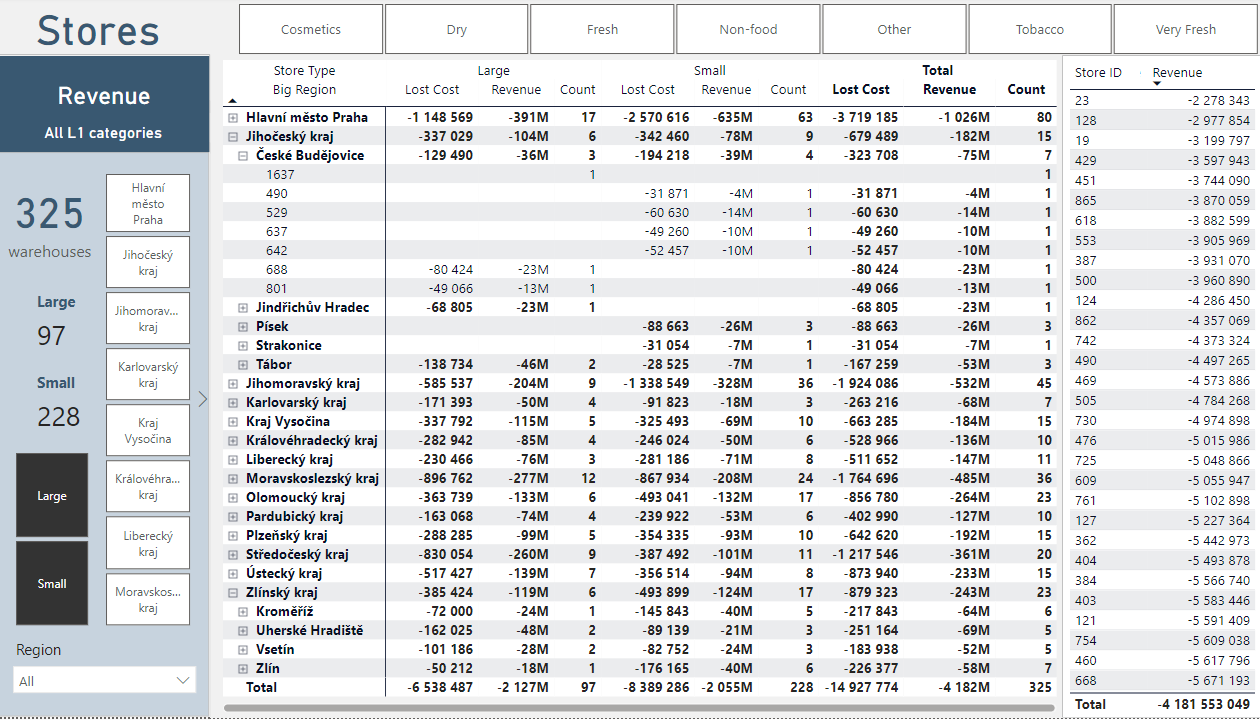
\includegraphics[width=\textwidth]{obrazky/PBI/stores.png}
    \caption{Power BI reporting pro zobrazení údajů o shrincích z pohledu prodejen.}
    \label{obr:PBI:stores}
\end{figure}


\section{Výsledky}
\label{sec:vizualizace:vysl}
